\chapter{Kết quả}
\label{Chapter5}

\emph{Chương này trình bày kết quả đề tài, bao gồm kết quả lựa chọn phần cứng, các công nghệ được sử dụng và các chức năng đã cài đặt được.}

\section{Công nghệ}

\subsection{Flutter}
Để xây dựng giao diện web cho hệ thống nhóm đã tiến hành tìm hiểu nhiều công nghệ xây dựng mobile như React Native\footnote{Xem thêm về React Native tại đây: \url{https://reactnative.dev/}}, Xamarin\footnote{Xem thêm về Xamarin tại đây: \url{https://docs.microsoft.com/en-us/xamarin/}}, Flutter\footnote{Flutter là một bộ công cụ giao diện người dùng để xây dựng ứng dụng cho nhiều nền tảng khác nhau như web, thiết bị di động, máy tính cá nhân với cùng một mã nguồn. Xem thêm về Flutter tại đây: \url{https://flutter.dev/}}.

Nhóm quyết định chọn Flutter vì các ưu điểm sau:
\begin{itemize}
    \item[--] Flutter là công nghệ mới nhưng có cộng đồng sử dụng đông đảo và phát triển nhanh, dễ dàng tìm được hỗ trợ nếu xảy ra lỗi
    \item[--] Bộ giao diện dựng sẵn của Flutter tuân thủ đầy đủ bộ quy tắc thiết kế giao diện Material Design\footnote{Bộ quy tắc thiết kế giao diện hiện đại và phổ biến của Google. Xem thêm về Material Design tại đây: \url{https://material.io/design}}, mang đến một giao diện hiện đại cho hệ thống
    \item[--] Flutter mang đến tính năng hot reload\footnote{Tính năng cho phép những thay đổi trong mã nguồn được hiển thị gần như lập tức trên giao diện}, kết hợp với bộ giao diện dựng sẵn và trình kiểm tra lỗi dễ sử dụng giúp quá trình phát triển nhanh chóng
\end{itemize}

\subsection{Snips NLU}
Snips-NLU - bộ công cụ trích xuất thông tin có cấu trúc từ các câu được viết bằng ngôn ngữ tự nhiên mã nguồn mở được viết bằng Python.
Đây là một bộ công cụ được sử dụng rộng rãi để phục vụ những nhà nghiên cứu hiểu ngôn ngữ tự nhiên - NLU (Natural Language Understanding) nhằm xây dựng một hệ thống hiểu được ngôn ngữ mà con người sử dụng. Các bài báo liên quan mà nhóm tìm hiểu được sử dụng trong đề tài được thực hiện trên bộ công cụ này. Mô hình huấn luyện được nhóm tự xây dựng và sử dụng công cụ này để huấn luyện.

\subsection{Flutter}
Để xây dựng giao diện ứng dụng cho hệ thống nhóm đã tiến hành tìm hiểu nhiều công nghệ xây dựng mobile như React Native\footnote{Xem thêm về React Native tại đây: \url{https://reactnative.dev/}}, Xamarin\footnote{Xem thêm về Xamarin tại đây: \url{https://docs.microsoft.com/en-us/xamarin/}}, Flutter\footnote{Flutter là một bộ công cụ giao diện người dùng để xây dựng ứng dụng cho nhiều nền tảng khác nhau như web, thiết bị di động, máy tính cá nhân với cùng một mã nguồn. Xem thêm về Flutter tại đây: \url{https://flutter.dev/}}.

Nhóm quyết định chọn Flutter vì các ưu điểm sau:
\begin{itemize}
    \item[--] Flutter là công nghệ mới nhưng có cộng đồng sử dụng đông đảo và phát triển nhanh, dễ dàng tìm được hỗ trợ nếu xảy ra lỗi
    \item[--] Bộ giao diện dựng sẵn của Flutter tuân thủ đầy đủ bộ quy tắc thiết kế giao diện Material Design\footnote{Bộ quy tắc thiết kế giao diện hiện đại và phổ biến của Google. Xem thêm về Material Design tại đây: \url{https://material.io/design}}, mang đến một giao diện hiện đại cho hệ thống
    \item[--] Flutter mang đến tính năng hot reload\footnote{Tính năng cho phép những thay đổi trong mã nguồn được hiển thị gần như lập tức trên giao diện}, kết hợp với bộ giao diện dựng sẵn và trình kiểm tra lỗi dễ sử dụng giúp quá trình phát triển nhanh chóng
\end{itemize}

\subsection{Flask Python}
Python ngày càng chứng minh ưu thế của mình trong việc xây dựng và triển khai nhiều loại ứng dụng khác nhau như web application, desktop application, Machine Leaning, Deep Learning….
Để xây dựng \ac{api} cho hệ thống và thuận tiện cho việc nghiên cứu, nhóm chúng em đã tiến hành tìm hiểu nhiều framwork để xây dựng trên Python như Flask\footnote{Xem thêm về Flask tại đây:\url{https://flask.palletsprojects.com}}, Django\footnote{Xem thêm về Django tại đây:\url{https://docs.djangoproject.com}}, Tornado \footnote{Xem thêm về Tornado tại đây: \url{https://www.tornadoweb.org}}, Pyramid\footnote{Xem thêm về Pyrmaid tại đây: \url{https://docs.pylonsproject.org/}}

Nhóm quyết định chọn Flask Python vì các ưu điểm sau:
\begin{itemize}
    \item[--] Đơn giản và dễ dàng sử dụng
    \item[--] Flask Python là micro web framework, không cần công cụ hoặc thư viện cụ thể, nó mang đến các chức năng tối giản nhưng có thể mở rộng cho các ứng dụng web.
    \item[--] Hỗ trợ xây dựng các API, web services, các ứng dụng web application cỡ vừa và nhỏ.
    \item[--] Flask cung cấp rất nhiều tài liệu từ cài đặt đến thực hiện và triển khai, từ hướng dẫn nhanh đến hướng dẫn chi tiết. Nguồn tài liệu tham khảo về Flask rất phong phú giúp dễ dàng tham khảo và tìm hiểu.
\end{itemize}

Theo đánh giá năm 2020 của JetBrains Python Developers Survey\footnote{Xem thêm tại đây: \url{https://www.jetbrains.com/lp/python-developers-survey-2020/}} thì Flask hiện là framework được sử dụng rộng rãi nhất, chiếm tới 46\% thị phần.  

\section{Một số chức năng chính đã cài đặt}

\subsection{Chức năng chỉ đường từ một đia điểm đến một địa điểm xác định}
\begin{figure}[htp]
    \centering
    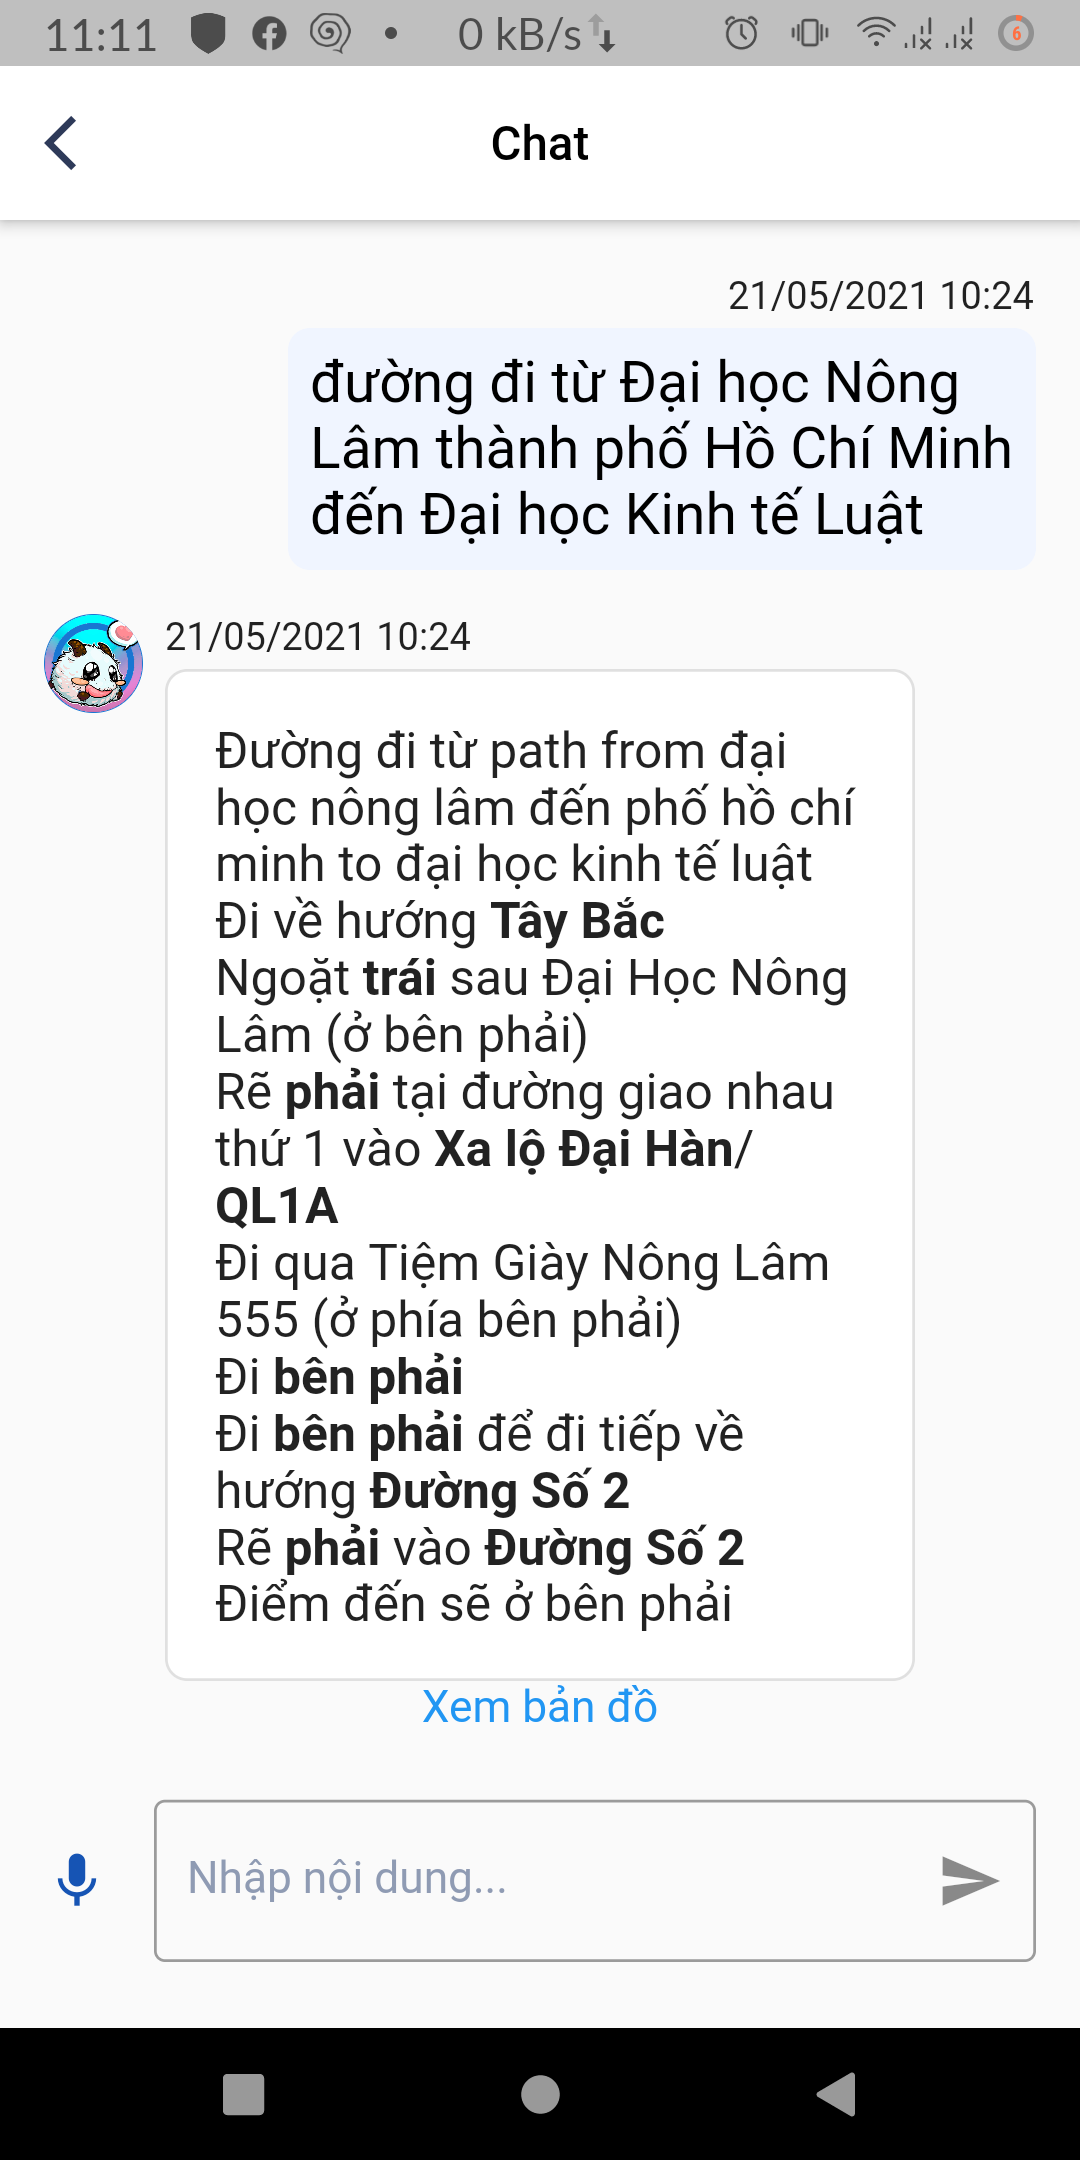
\includegraphics[width=10cm]{images/Screen-chat.png}
    \caption{Màn hình trò chuyện}
    \label{fig:screen-chat}
\end{figure}

\begin{figure}[htp]
    \centering
    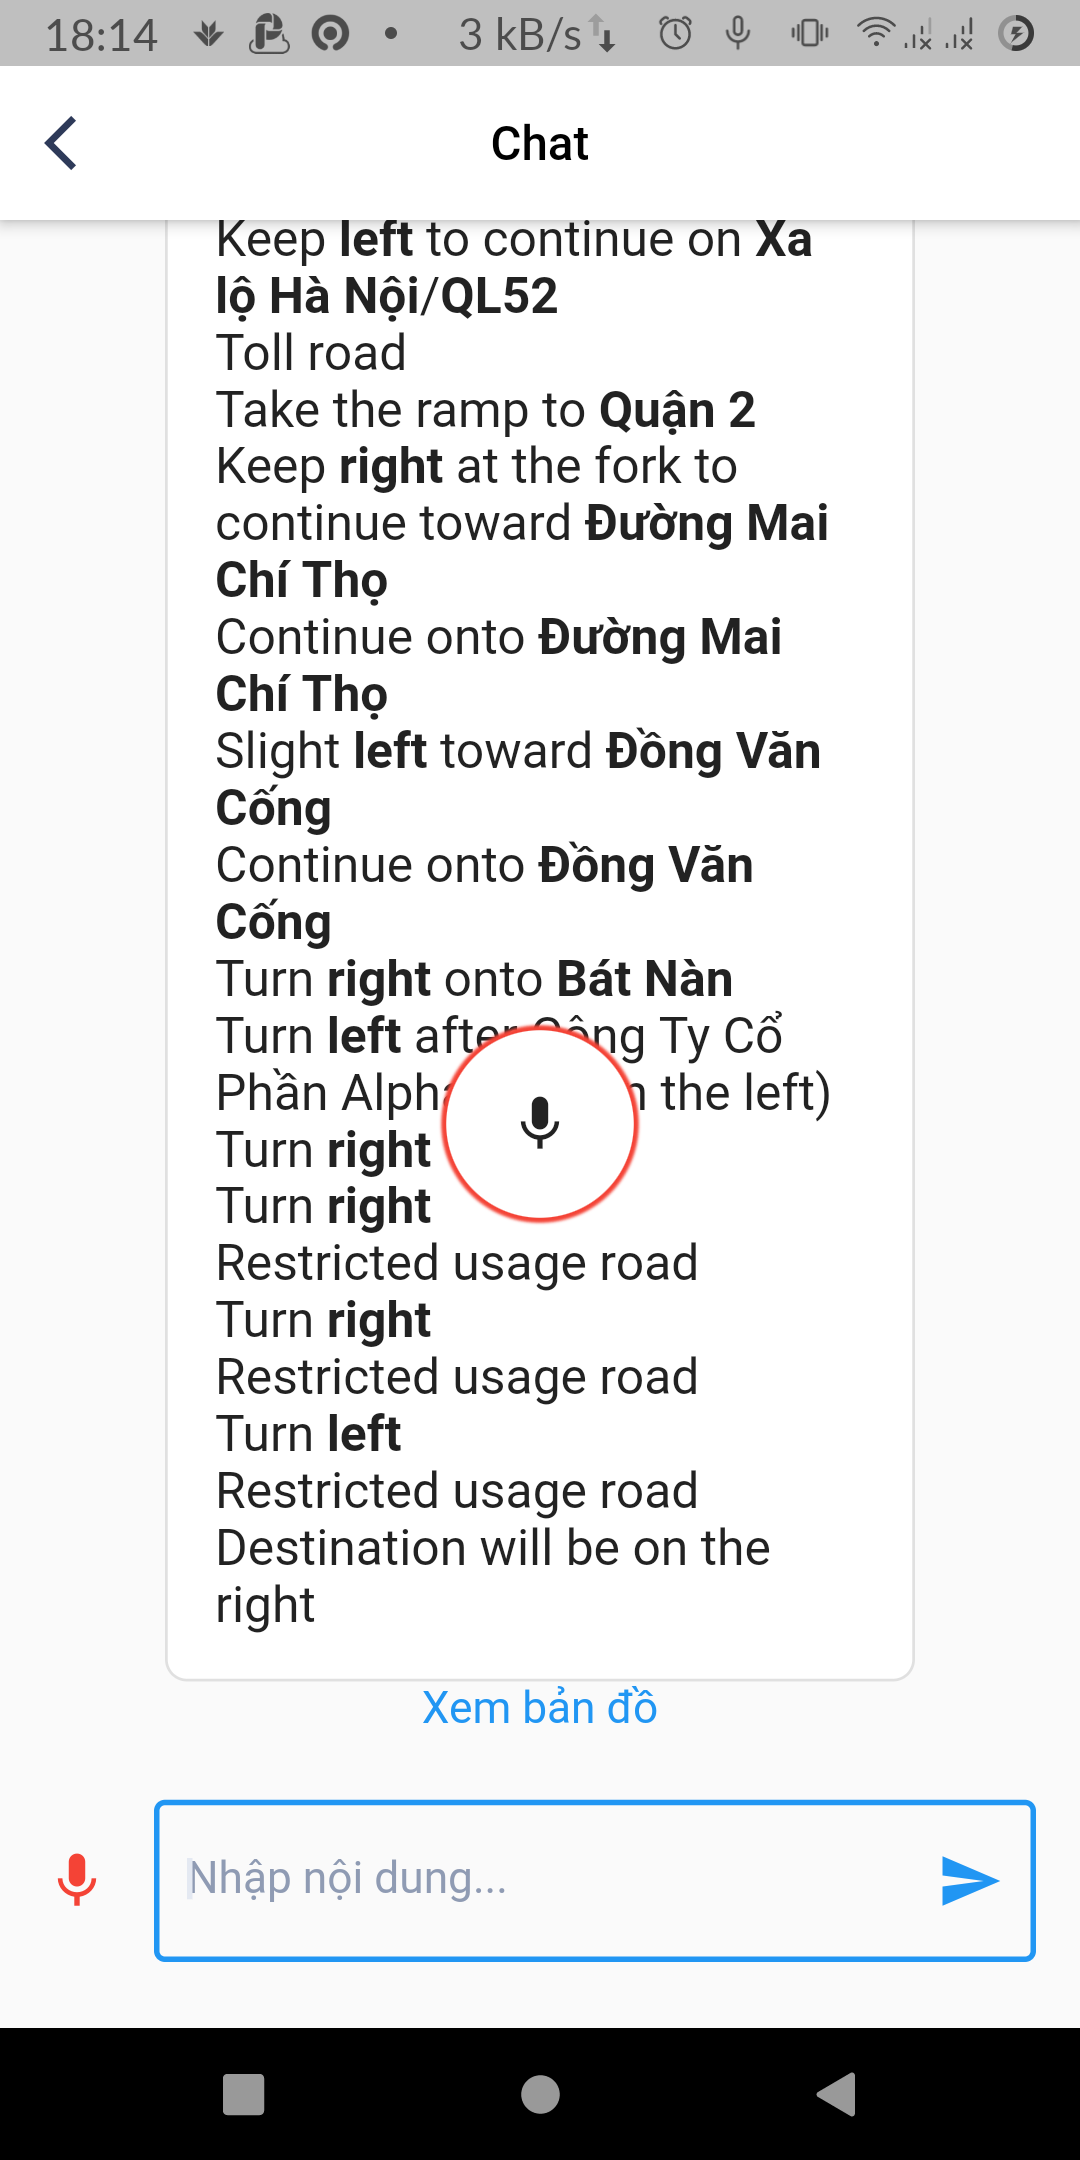
\includegraphics[width=10cm]{images/Screen-record.png}
    \caption{Màn hình thể hiện đang ghi âm}
    \label{fig:screen-record}
\end{figure}

\begin{figure}[htp]
    \centering
    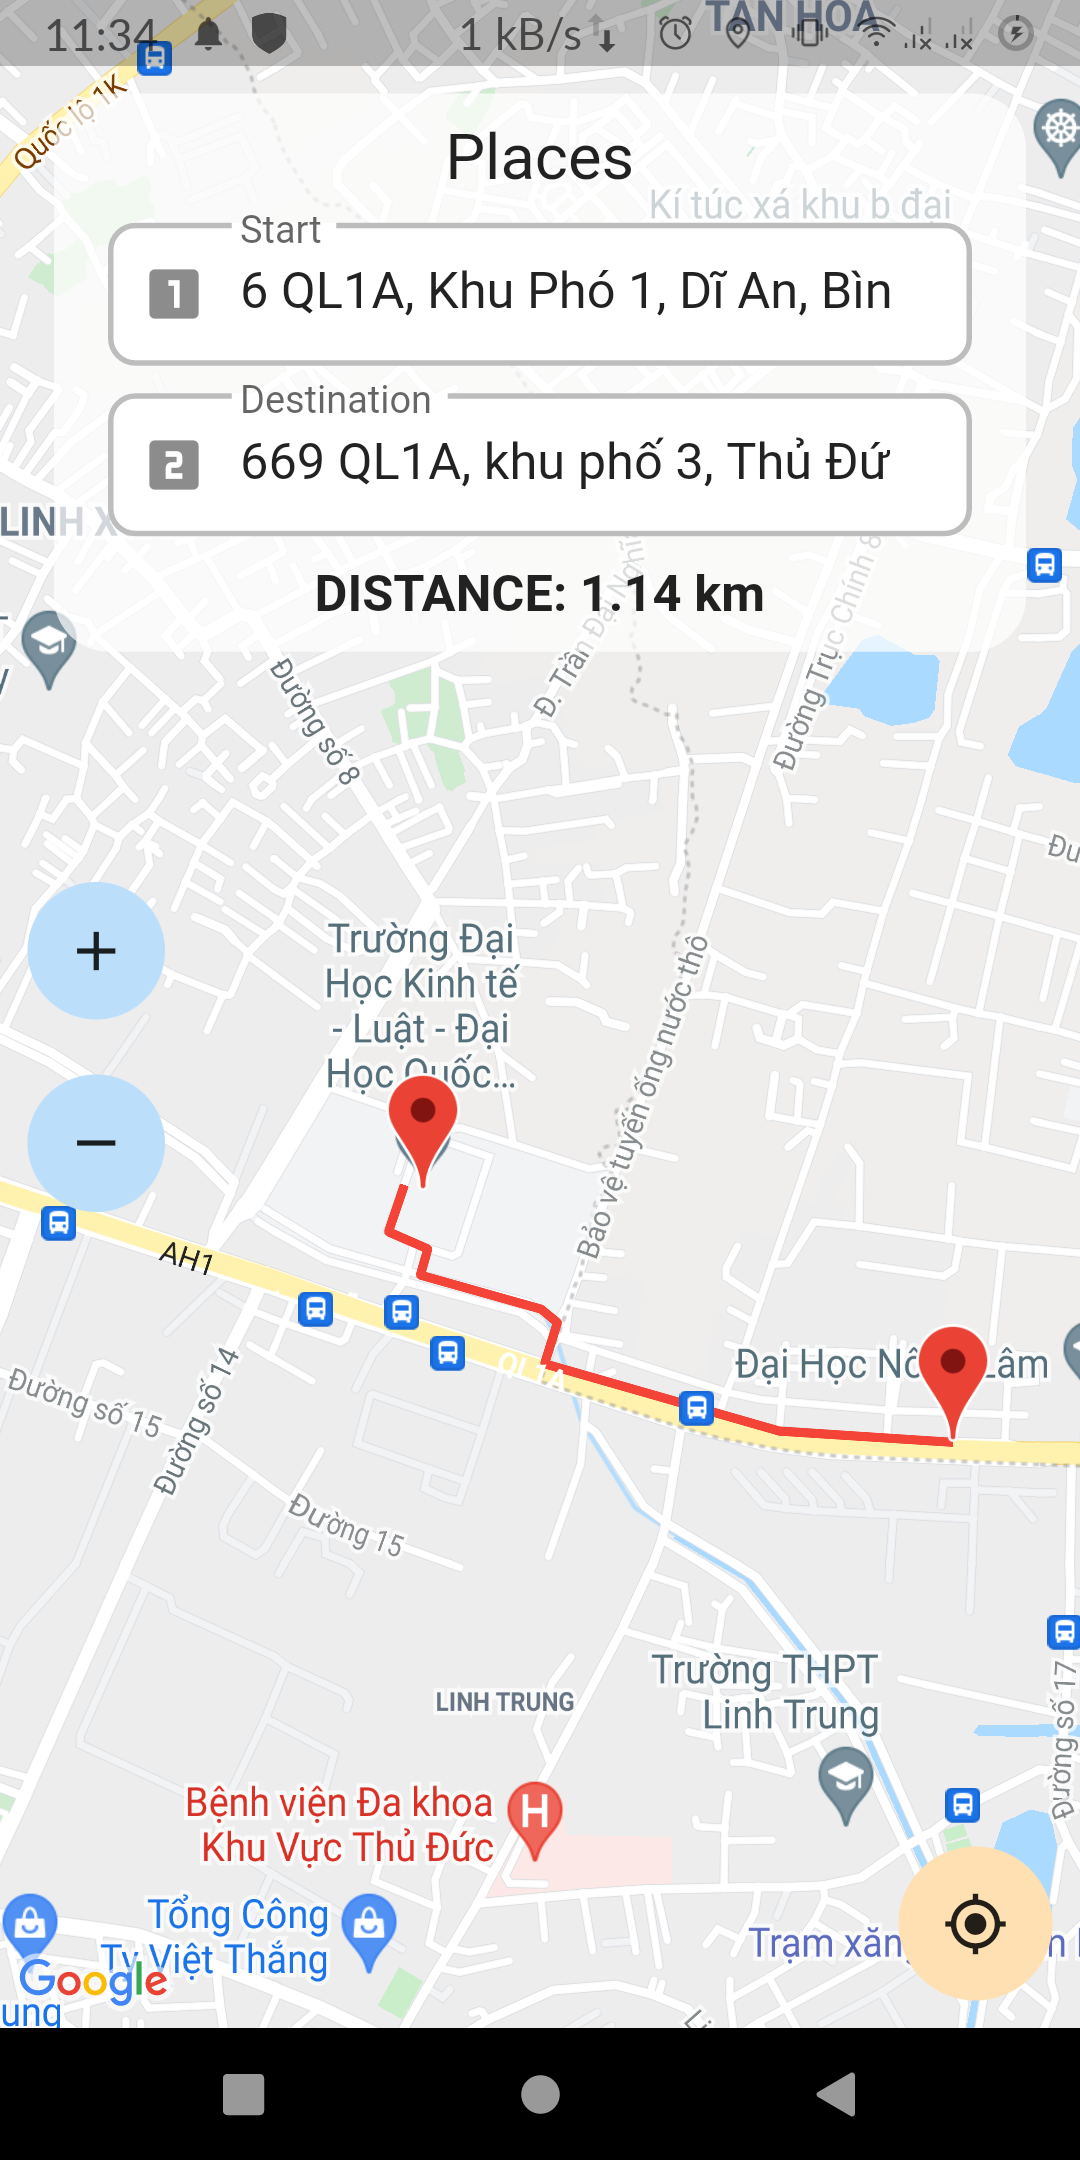
\includegraphics[width=10cm]{images/Screen-Map.png}
    \caption{Màn hình chỉ đường}
    \label{fig:screen-map}
\end{figure}

Chức năng chỉ đường từ một địa điểm đến một địa điểm xác định cho phép người dùng có thể hỏi đường bằng văn bản và giọng nói.
\begin{itemize}
    \item Hỏi đường bằng văn bản: Người dùng nhập 1 câu hỏi bằng văn bản vào ứng dụng. VD: “Đường đi từ UBND thành phố Thủ Đức đến Công An thành phố Thủ Đức”. Bấm nút gửi
    \item Hỏi đường bằng giọng nói: Người dùng ấn giữ icon ghi âm và nói 1 câu vào ứng dụng. VD: “Đường đi từ UBND thành phố Thủ Đức đến Công An thành phố Thủ Đức”
    \item Ứng dụng hiển thị câu trả lời bằng văn bản lên màn hình, chuyển văn bản thành âm thanh và phát lên.
    \item Button "Xem đường đi" dùng để chuyển sang màn hình chỉ đường của bản đồ giúp người dùng có thể xem đường đi một cách cụ thể hơn.
    \item Ở màn hình bản đồ, bạn có thể xem được đường đi cụ thể mà bạn vừa yêu cầu và khoảng cách sẽ được hiển thị lên bản đồ. Bạn có thể phóng to, thu nhỏ bản đồ và có thể xem vị trí hiện tại của mình.
\end{itemize}